\section{Results}

Partition Examples: Without any partitioning operation, the inner and outer boundary of of a shell model needs to be filled by a huge amount of support materials in order to guarantee a fine surface quality. See Figure \ref{fig:dear-simulation} (a-b) for an illustration of the sculpture model, both its inner and outer surface require significant amount of support in order not to be collapsed during the printing process; while our approach only keeps all cylindrical shells that are free of support (Figure \ref{fig:dear-simulation} (c-d)).

\begin{figure}[tbp]
  \centering
  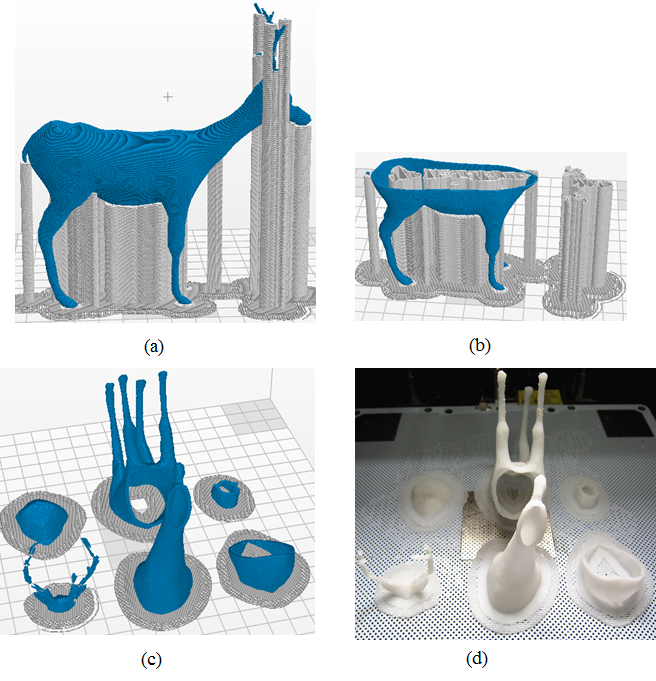
\includegraphics[width=\linewidth]{figs/dear-simulation.png}
  \caption{\label{fig:dear-simulation}%
           An illustration of the sculpture model under the 3D printing software Z-suite as $\theta = 20^{\circ}$; (a) the full model; (b) an intermediate step of the simulation; (c) the simulation result of our partitioned shell models; (d) the 3D printed shell parts free of support.}
\end{figure}

We have run our algorithm on various natural or man-made models, and some of the results are presented as follows:

\begin{figure}[tbp]
  \centering
  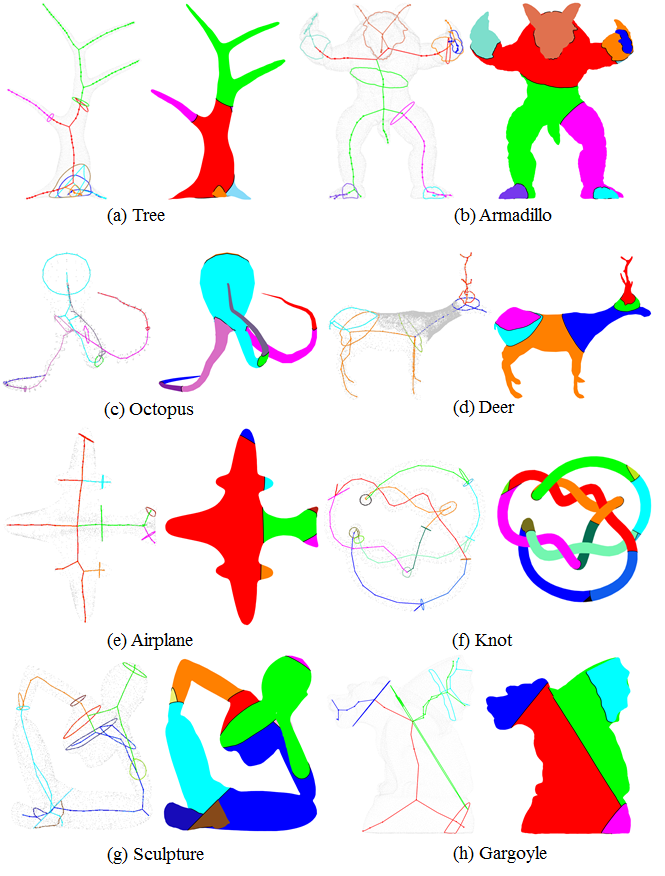
\includegraphics[width=0.45\textwidth]{figs/programming.png}
  \caption{\label{fig:programming}%
           Partition examples as $\theta = 70^{\circ}$. The printing direction of each part is orthogonal to its base (shown in the same color as the part)}
\end{figure}

Experimental Validation: We validated our approach by a set of printing experiments on Zortrax desktop printer, a kind of FDM machine that allows a printing layer thickness of 0.09mm , this is also the layer thickness we used in the printing experiments. The experiments are based on the choice of $\theta = 70^{\circ}$, i.e., all overhangs with an angle of no larger than $20^{\circ}$ with respect to the build platform are given support structures. Zortrax provides a built-in 3D printing software called \emph{Z-suite} can automatically counts the filament of the print material (in meters) and an estimate of the weight of the print material. The following table summarizes the printing material and time costs by the original models and the partitioned models. Our approach significantly reduces both the printing material and time as the skeleton-based partition reduces both the supported materials inside and outside the models.


\begin{table*}[htb]

\begin{footnotesize}

\begin{center}

    \begin{tabular}{p{1cm} p{2cm} p{2cm} p{1.6cm} p{1.6cm} p{1.5cm} p{1.5cm} p{1.5cm} p{1.5cm}}

    \hline

     Models& Print material (original)& Print time (original)& Number of parts (skeleton partition)& Number of parts (mesh partition)& Print material (partition)& Print time (partition)& Material save (\%) &Time save(\%)\\ \hline
     Tree& 8.4m (20g)& 6h 32min &6 & 8 &5.19(12g) & 4h 2min & 38.2143 &38.2653\\ \hline
     Armadillo& 11.26m (27g)& 7h 30min &9 & 10  &4.65(11g) & 3h 30min & 58.7034 &53.3333\\ \hline
     Octopus& 12.82m (31g)& 10h 2min &5 & 9  &8.75(21g) &6h 51min & 31.7473 &31.7276\\ \hline
     Deer& 20.1m (48g)& 15h 8min &4 & 6  &8.89(21g) &5h 25min & 55.7711 &64.207\\ \hline
     Airplane& 11.56m (28g)& 6h 34min &5 & 7 &5.24(12g) &3h 10min & 54.6713 &51.7766\\ \hline
     Knots& 20.87m (50g)& 16h 50min &10 & 15 &12.38(29g) &11h 20min & 40.6804 &32.6733\\ \hline
     Sculpture& 23.68m (56g)& 18h 59min &4 & 10 &16.35(39g) &11h 23min & 30.9544 &40.0351\\ \hline
     Gargoyle& 8.76m (21g)& 6h 49min &4 & 5 &5.16(12g) &3h 48min & 41.0959 &44.2543\\ \hline

  \hline

    \end{tabular}

\end{center}

\end{footnotesize}

\caption{Statistics showing the print material, print time and partition number of the printed models.}\label{tab:ertms:summary}

\end{table*}

The improved algorithm was implemented with C++ on a PC with Intel i7-4790 and 8 GB RAM. The running time of processing the models are summarized in Table \ref{tab:ertms:time}.

\begin{table*}[htb]

\begin{footnotesize}

\begin{center}

    \begin{tabular}{p{2.3cm} p{1.45cm} p{1.45cm} p{1.5cm} p{1.5cm} p{1.5cm} p{1.5cm} p{1.5cm}p{1.5cm}}

    \hline

     Models& Tree& Armadillo& Octopus& Deer& Airplane& Knots &Sculpture & Gargoyle\\ \hline
     number of vertices & 11443   & 34594   & 1343    & 8917  & 15485 & 2904    & 5979    &25002 \\ \hline
     running time(s)    &197.1732 & 311.559 & 97.1395 &90.618 &88.744 & 92.4798 &74.2186  &199.893 \\ \hline

  \hline

    \end{tabular}

\end{center}

\end{footnotesize}

\caption{The running time of processing the models.}\label{tab:ertms:time}

\end{table*}




\begin{figure}[tbp]
  \centering
  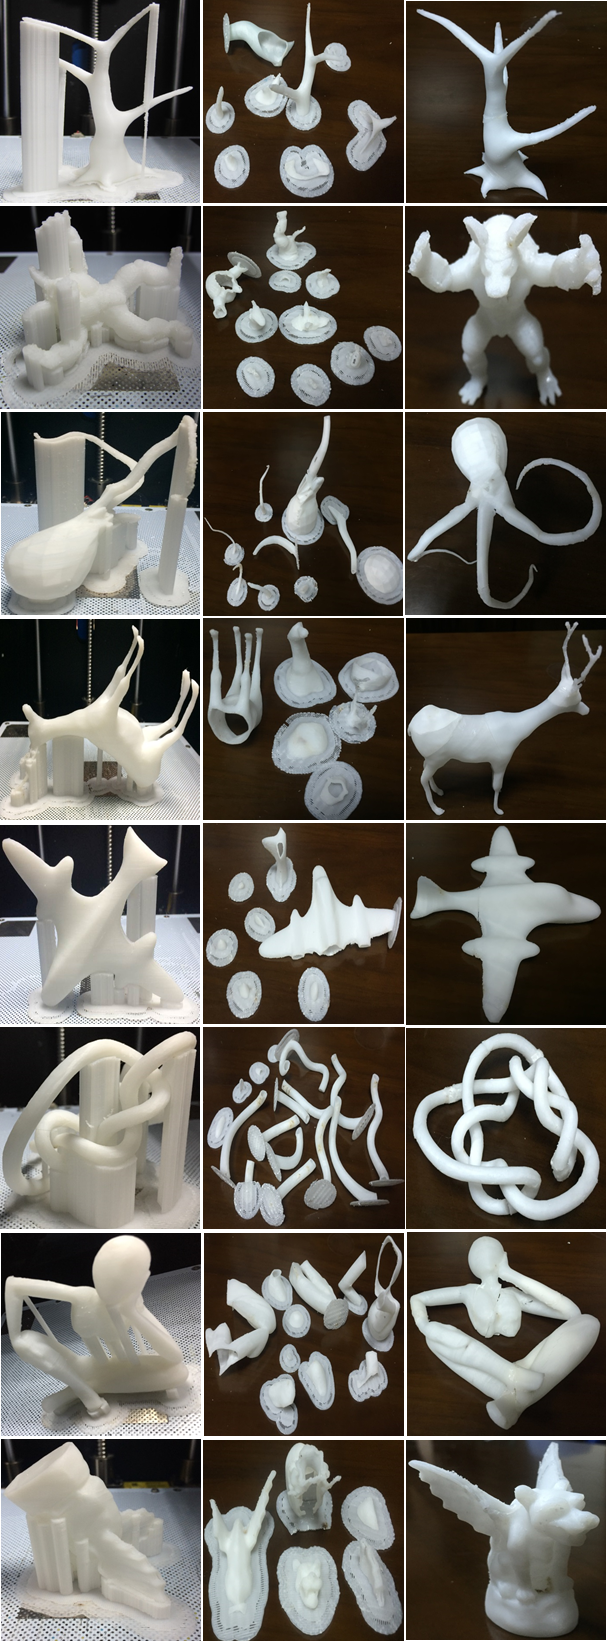
\includegraphics[width=0.48\textwidth]{figs/experiment.png}
  \caption{\label{fig:experiment}%
           A comparison between printing of original shell models and our partitioned models.}
\end{figure}


 Figure \ref{fig:experiment} shows the comparison of the printing effects of the original models and our partitioned models. Due to the limit of the current technology, any FDM printer requires a small amount of supporting bed for holding the printed model on the printing platform, other printing techniques such as SLA, SLM and SLS may avoid the use of these supporting beds. Therefore, our approach guarantees support-free to the most extent for all exiting printing techniques.

\hl {[Evaluations: how close we are to the global optimum][Limitations: discussion about 1. the strength of our interior, -- future work. 2. cut through salient regions -- hard to balance. etc]}

Since the problem of partitioning the skeleton graph into the least number of support-free subgraphs is NP-hard, it is impossible to obtain an optimal result in polynomial time. However, from Table \ref{tab:ertms:summary}, we can conclude that the partition result for the skeletons are small enough. Particularly, which arcs to be taken into a subgraph and the taking sequence significantly affect the final partition result. Further, our current approach of partitioning tries to find a node as a root of a subgraph, while in general it is possible that the subgraph is unrooted. For example, in Figure \ref{fig:unrooted}, under the angle constraint of $\theta = 70{\circ}$, the tree skeleton can be taken as a whole printable graph while our algorithm would take node $v$ as a root for the upper and lower parts of the tree respectively. Future research can be elaborated along this line. But how the general unrooted subgraphs are taken efficiently other than  searching in an exhaustive combinatorial manner to form a minimum set of subgraphs is unknown.

\begin{figure}[tbp]
  \centering
  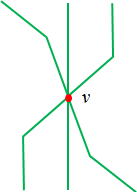
\includegraphics[width=0.2\textwidth]{figs/unrooted.png}
  \caption{\label{fig:unrooted}%
           An illustration of a tree skeleton that satisfies the angle constraint but is taken as two subgraphs by our algorithm.}
\end{figure}

%However, we can evaluate the effectiveness of our approach by judging the topology of some simple models and evaluate how close our partition is from a potential optimal result. For example, from Figure \ref{fig:ex1}, under the requirement of $\theta = 70^{\circ}$, ignoring the tinny detailed geometric features we can observe that an optimal partition of the deer model requires at least $4$ cuts: the tail, the chunk including the legs, the neck, and the head and the horn. Our approach provides a partition of 4 cuts, which is almost near the optimal. Further, from the appearance of the gargoyle model (the last row of Figure \ref{fig:experiment}), we can see that an optimal cutting should have the following 4 parts: the head, two wings, and the remaining parts. Our partition results in 5 parts, which is very close to the potential optimal partition.

%Our approach is devoted to shell models, it can also be applied to cutting solid models without any problem. However, our approach suffers from a few limitations: for shell models, the thickness of the shells need to be large enough such that no serious deformation is caused during the assembling process. However, the problem of setting the minimum thickness of the model for various parts of the model is non-trivial, and our current work is restricted to a uniform setting of the shell thickness whose value is determined by an error-and-trial process. Further, the strength guarantee is not elaborated in this work, a possible solution is to use the algorithm in \cite{WangWYLTTDCL13} that distributes the least amount of materials for constructing a truss frame beneath the skin. Finally, our approach may allow a cut that passes through a salience region, which may hurt the appearance of the model. We found that it is difficult to make a balance between the saliency and the minimal cutting length as well as the minimal cutting numbers. A potential future research is to take care of salience region during graph partition. Finally, as a trade-off, a spatially curved cut might be a consideration to alleviate the salience problem.
